\documentclass[a4paper,titlepage]{article}


\usepackage{arxiv}
\usepackage[utf8]{inputenc} % allow utf-8 input
\usepackage[T1]{fontenc}    % use 8-bit T1 fonts % for underscore char
\usepackage{hyperref}       % hyperlinks
\usepackage{url}            % simple URL typesetting
\usepackage{booktabs}       % professional-quality tables
\usepackage{amsfonts}       % blackboard math symbols
\usepackage{nicefrac}       % compact symbols for 1/2, etc.
\usepackage{microtype}      % microtypography
\usepackage{listings}
\usepackage{graphicx}
\usepackage{subcaption}
\usepackage{color}
\usepackage[svgnames]{xcolor}
\usepackage[title]{appendix}

\newcommand*{\fullref}[1]{\hyperref[{#1}]{\mbox{\autoref*{#1}~}``\nameref*{#1}''}}
\newcommand{\code}[1]{\mbox{\lstinline{#1}}}
\lstset{frame=tb,
escapeinside={(*@}{@*)},
language=C++,
alsolanguage=Python,
aboveskip=3mm,
belowskip=3mm,
showstringspaces=false,
columns=flexible,
basicstyle={\small\ttfamily},
numbers=left,
numberstyle=\color{gray},
keywordstyle=\color{blue},
commentstyle=\color{green},
stringstyle=\color{mauve},
breaklines=true,
breakatwhitespace=true,
tabsize=3,
upquote=true
}

\title{Loop Programming Practices that Simplify Quicksort Implementations}


\author{Shoupu Wan \\
\texttt{wanshoupu@gmail.com} \\
}

\begin{document}
    \maketitle

    \begin{abstract}
        Quicksort algorithm with Hoare's partition scheme is traditionally implemented with
        nested loops.
        In this article, we present loop programming and refactoring techniques
        that lead to simplified implementation for Hoare's quicksort algorithm consisting of a
        single loop.
        We believe that the techniques are beneficial for general programming and may be used for
        the discovery of more novel algorithms.
    \end{abstract}


    % keywords can be removed
    \keywords{Quicksort \and Loop rotation \and Nested loop thinning \and Cascading conditional
    \and Sentinel}


    \section{Introduction}\label{sec:introduction}
    Loops are one of the most widely used programming constructs featured
    in almost all programming languages.
    A loop is an productivity amplifier.
    With nominal overheads (\textit{e.g.}, state-registering variables, \textit{etc.}),
    the static body of a loop can be reused for unlimited number of times.


    A key building block as loop, one would suppose its best practices should have been widely
    known.
    On the opposite, however, the best practices for loop has been so largely ignored that
    haphazardly constructed loops with duplication issues is not uncommon even in production code.
    Common problems in loop programming include, but are not limited to, duplicate code, nested
    loops, leaky loop variables, and oversized initialization.
    I will explain each of them next.


    Duplicate code here refers to duplication between code in the loop body and code before (after)
    the loop.
    It is the biggest problem in loop programming and is the most common root causes for bugs.
    Duplicate code anywhere is bad.
    But duplicate code of this type is harder to realize or get rid of.


    Uses of nested loops are sometimes controversial.
    Many readers are ready to argue about this.
    Anyhow, what is wrong with nested loop?
    %    The use of nested loops in many occasions seems to be reasonable, necessary,
    %    and at least harmless at first sight.
    %    But unfortunately this point of view does not stand for long.
    For almost all cases, nested loops bring complexity rather than convenience,
    obstruct readability rather than facilitating it.
    It turns what could have been coded as different components into monolithic mess and
    discourages code reusing.
    deepen the coupling rather than reducing it and discourage code reusability rather than encouraging it.


    Loop variables refers to variables used to register loop state.
    Many developers rely on exposed variable(s) to implicitly pass information from loop to
    subsequent program.
    However, uncontrolled exposure of loop variable to subsequent code is a violation of the
    encapsulation principle.
    While sometimes convenient, it usually does more harm than good.


    Loop initialization is the prelude code needed for instantiating initial loop state.
    It should be small and light-weight.
    rather than light-weight, succinct ones.
    However unseasoned programmers may code disproportionally heavy initializations.
    With due skills and perseverance, loop initializations can be made succinct one-liner.


    It is beyond the scope of this article to address all the topics.
    Instead we will focus on duplicate code and nested loops.
    We will present two pillar loop programming techniques---`loop rotation' and `Nested loop
    thinning' which I found are effective in fighting against above programming foes.
    These are the two pillars for loop programming.
    Proper use of them help developers avoid commonly made mistakes.


    We have tried these techniques on several case studies.
    Particularly, we will apply them to simplify traditional quicksort algorithm to prove the
    effectiveness of these techniques---the implementation of quicksort algorithms.
    First invented in 1960, quicksort has been studied and analyzed well over the
    years\cite{Hoare1961,Hoare1962,sedgewick:1978,Bentley:1986:PP}.
    As one of the earliest `divide-n-conquer` algorithms, quicksort has become the
    \textit{de facto} sorting algorithm in practice for its excellent expected performance.
    Recently named one of the top $10$ algorithms of $20$th century, quicksort has a
    profound influence on the history of programming\cite{top10algorithm:2000}.


    We will walk you through the multi-stage refactor process that leads to the discovery of a
    brand-new implementation of Hoare's quicksort algorithm.
    We use Python as the working language in this article.


    \section{Loop Rotation}\label{sec:loop-rotation}
    \begin{figure}[htb]
    \centering
    \begin{subfigure}{.3\textwidth}
        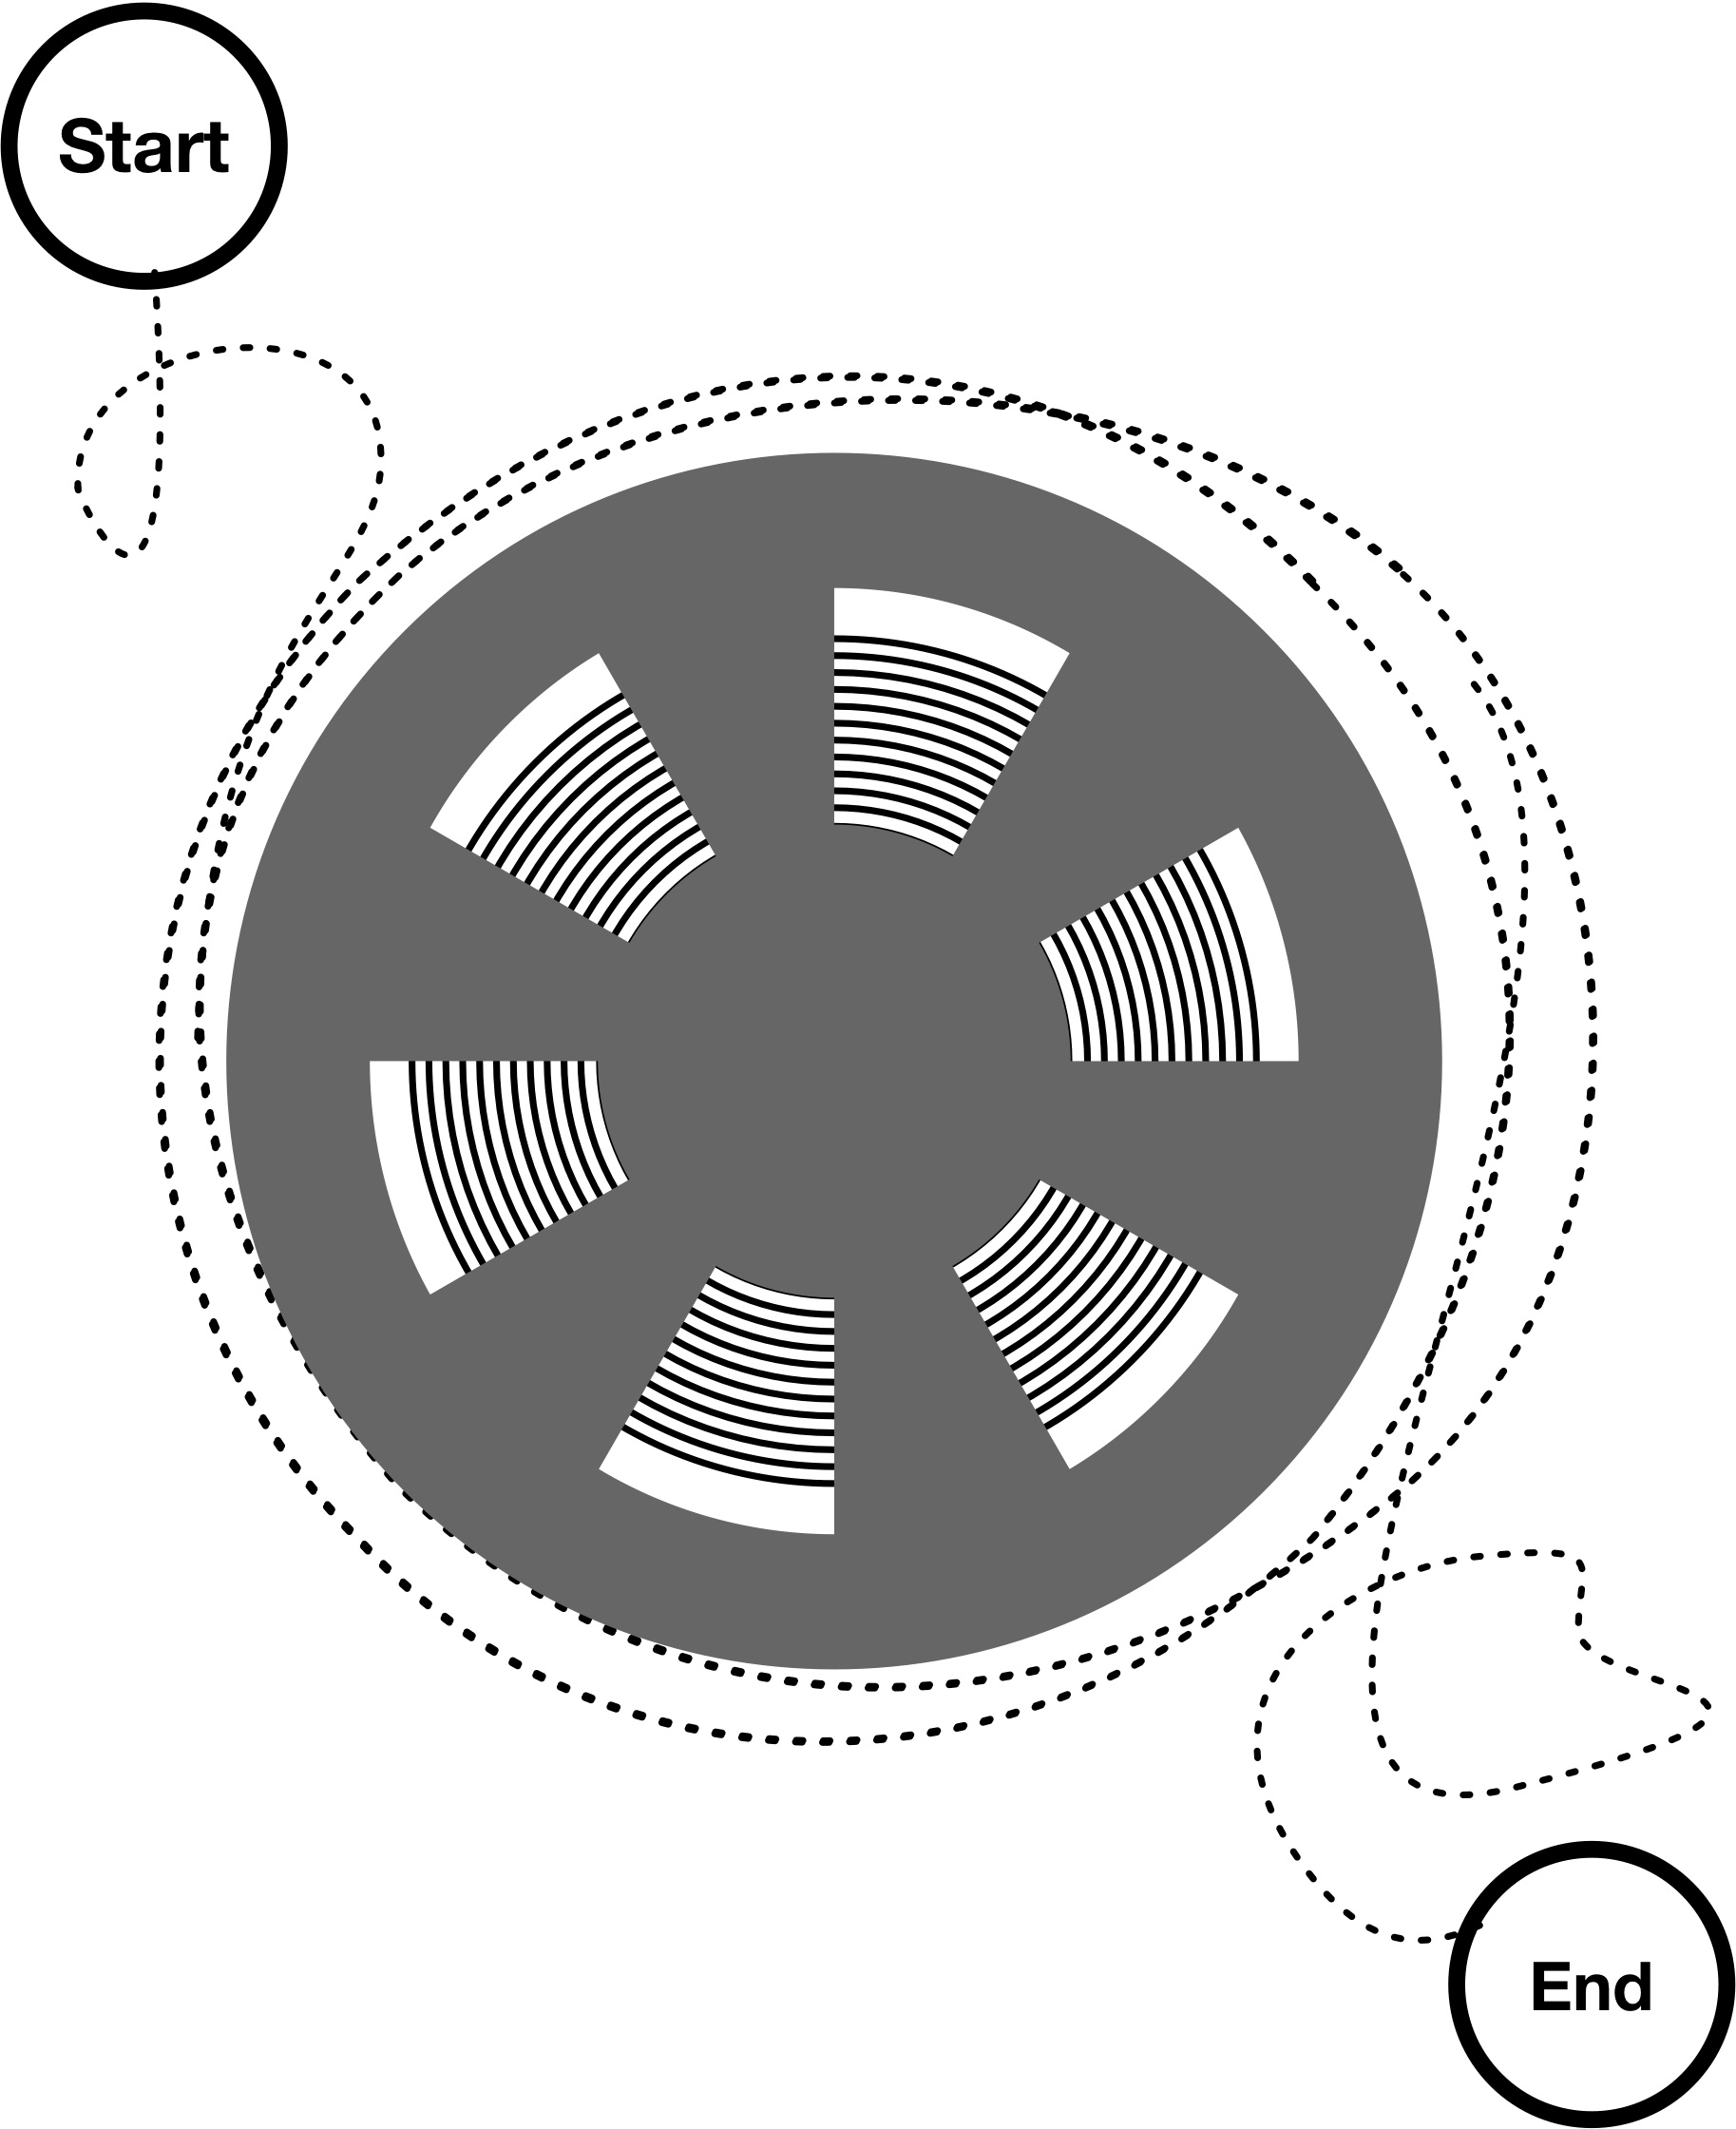
\includegraphics[width=\textwidth]{loose-spool.jpg}
        \caption{\label{fig:loose-spool}}
    \end{subfigure}
    \begin{subfigure}{.3\textwidth}
        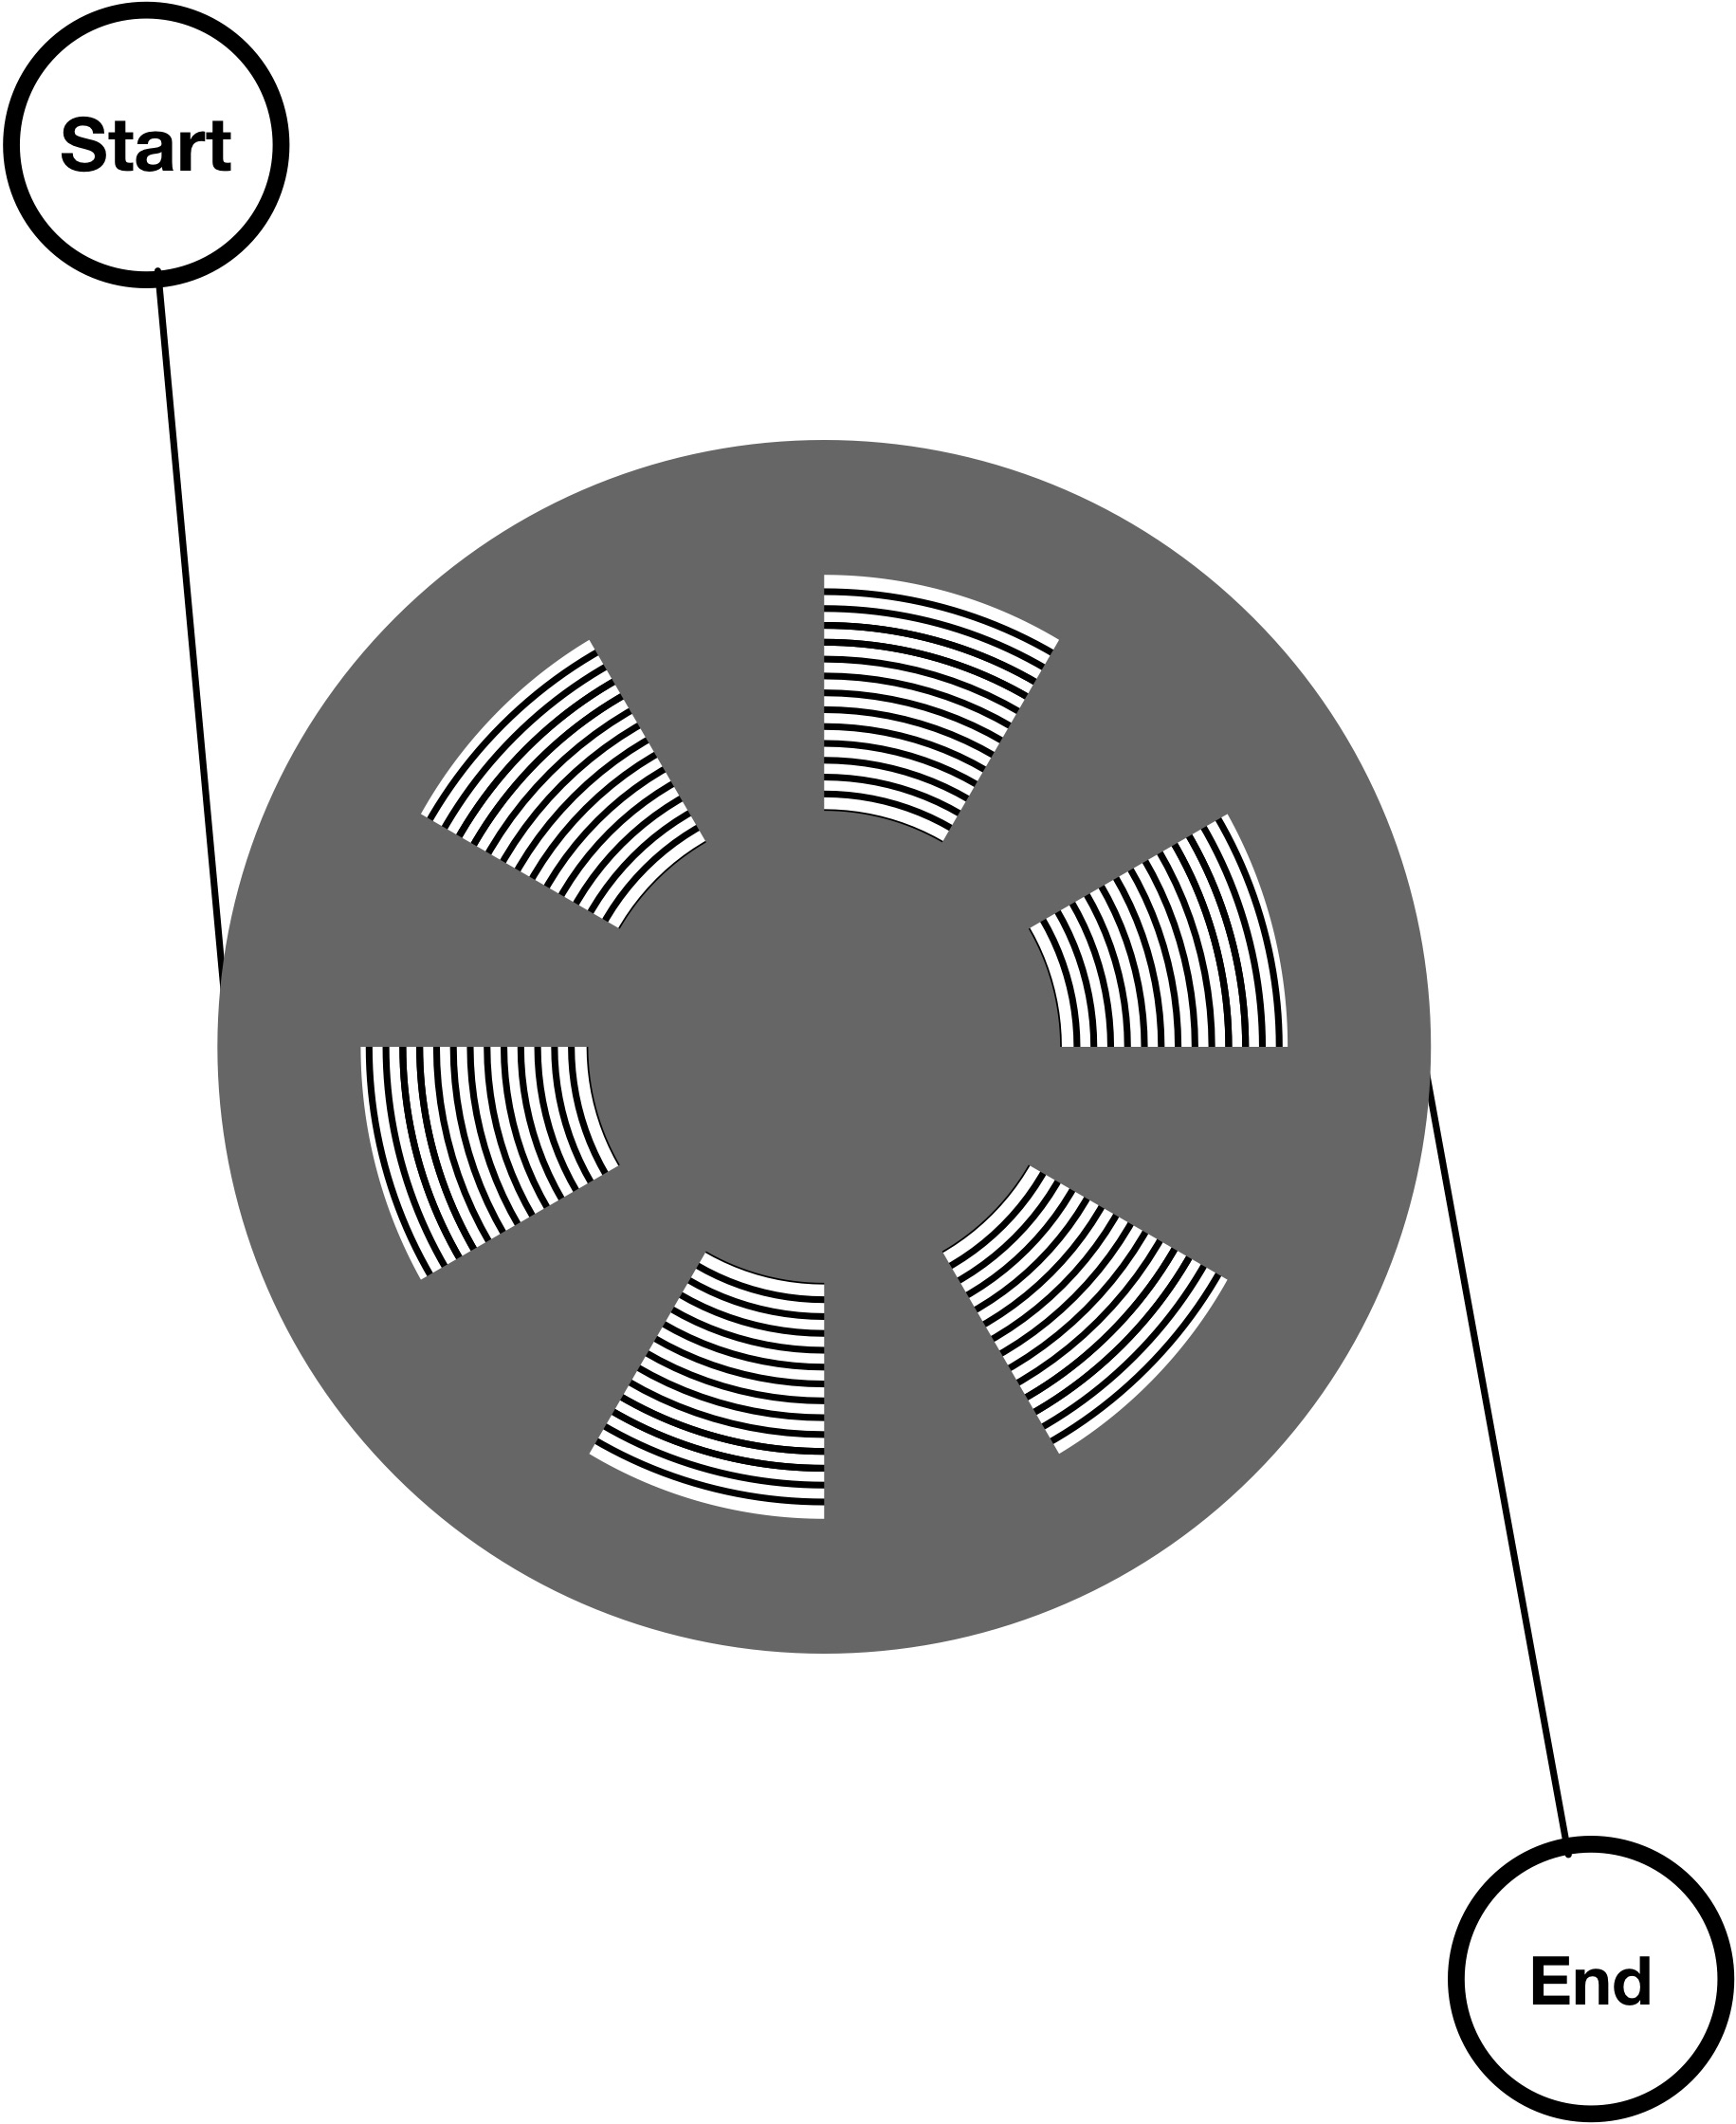
\includegraphics[width=\textwidth]{tight-spool.jpg}
        \caption{\label{fig:tight-spool}}
    \end{subfigure}
    \caption{\label{fig:spool-loop} Using spool as a metaphor for loop in program,
    duplicate code around a loop would be like tightening messy yarns into neat spool.
    `Loop rotation' can be pictorially depicted as winding up loose yarns onto a spool.
    \protect\subref{fig:loose-spool}: Duplicate, sloppy code is analogous to loose, unorganized
    yarn around a spool.
    \protect\subref{fig:tight-spool}: A neat loop is analogous to a tidy spool.}
\end{figure}


Coming with the productivity amplification power is the coding complexity of loops.
There are two key observations about loops.
First, a loop seldom lives in vacuum.
Loops are often used as an embedded subunits in a program just like an organelle in a living cell.
So it has to get along with its neighbors.
As a result, a large part of loop programming is to ``fit it in''.
Secondly, there are many moving parts in a loop construct and they are tightly coupled, changes in
one necessarily demand changes in others.
As we discussed in ~\autoref{sec:introduction}, the biggest problem with loop programming is
duplicate code in and around the loop.
The foremost goal in implementing loop is to reduce duplicate code.
`Loop rotation' is an important technique for that purpose.


As a helpful analogy, it is beneficial to visualize a loop construct as a spool.
Loops are to program as spools are to yarn---just as spools are used to organize yarn, loops are
invented to organize program.
From this perspective, the `loop rotation' process to coalesce duplicate code is analogous to
wind up loose and messy yarn into a tidy spool (~\autoref{fig:spool-loop}).


Additionally, a loop may be pictured as a Ferris wheel, a carousel and so on among which
the shared property is the symmetry with respect to circular shifts.
Aside from the point of entrance and one or more exits, a loop may be mathematically
represented by a circular sequence, that is, a sequence with rotational symmetry.
One can thus take this rotational degrees of freedom to one's advantage to decide where
to enter and where to exit the loop.


\begin{figure}[htb]
    \centering
    \begin{subfigure}{.3\textwidth}
        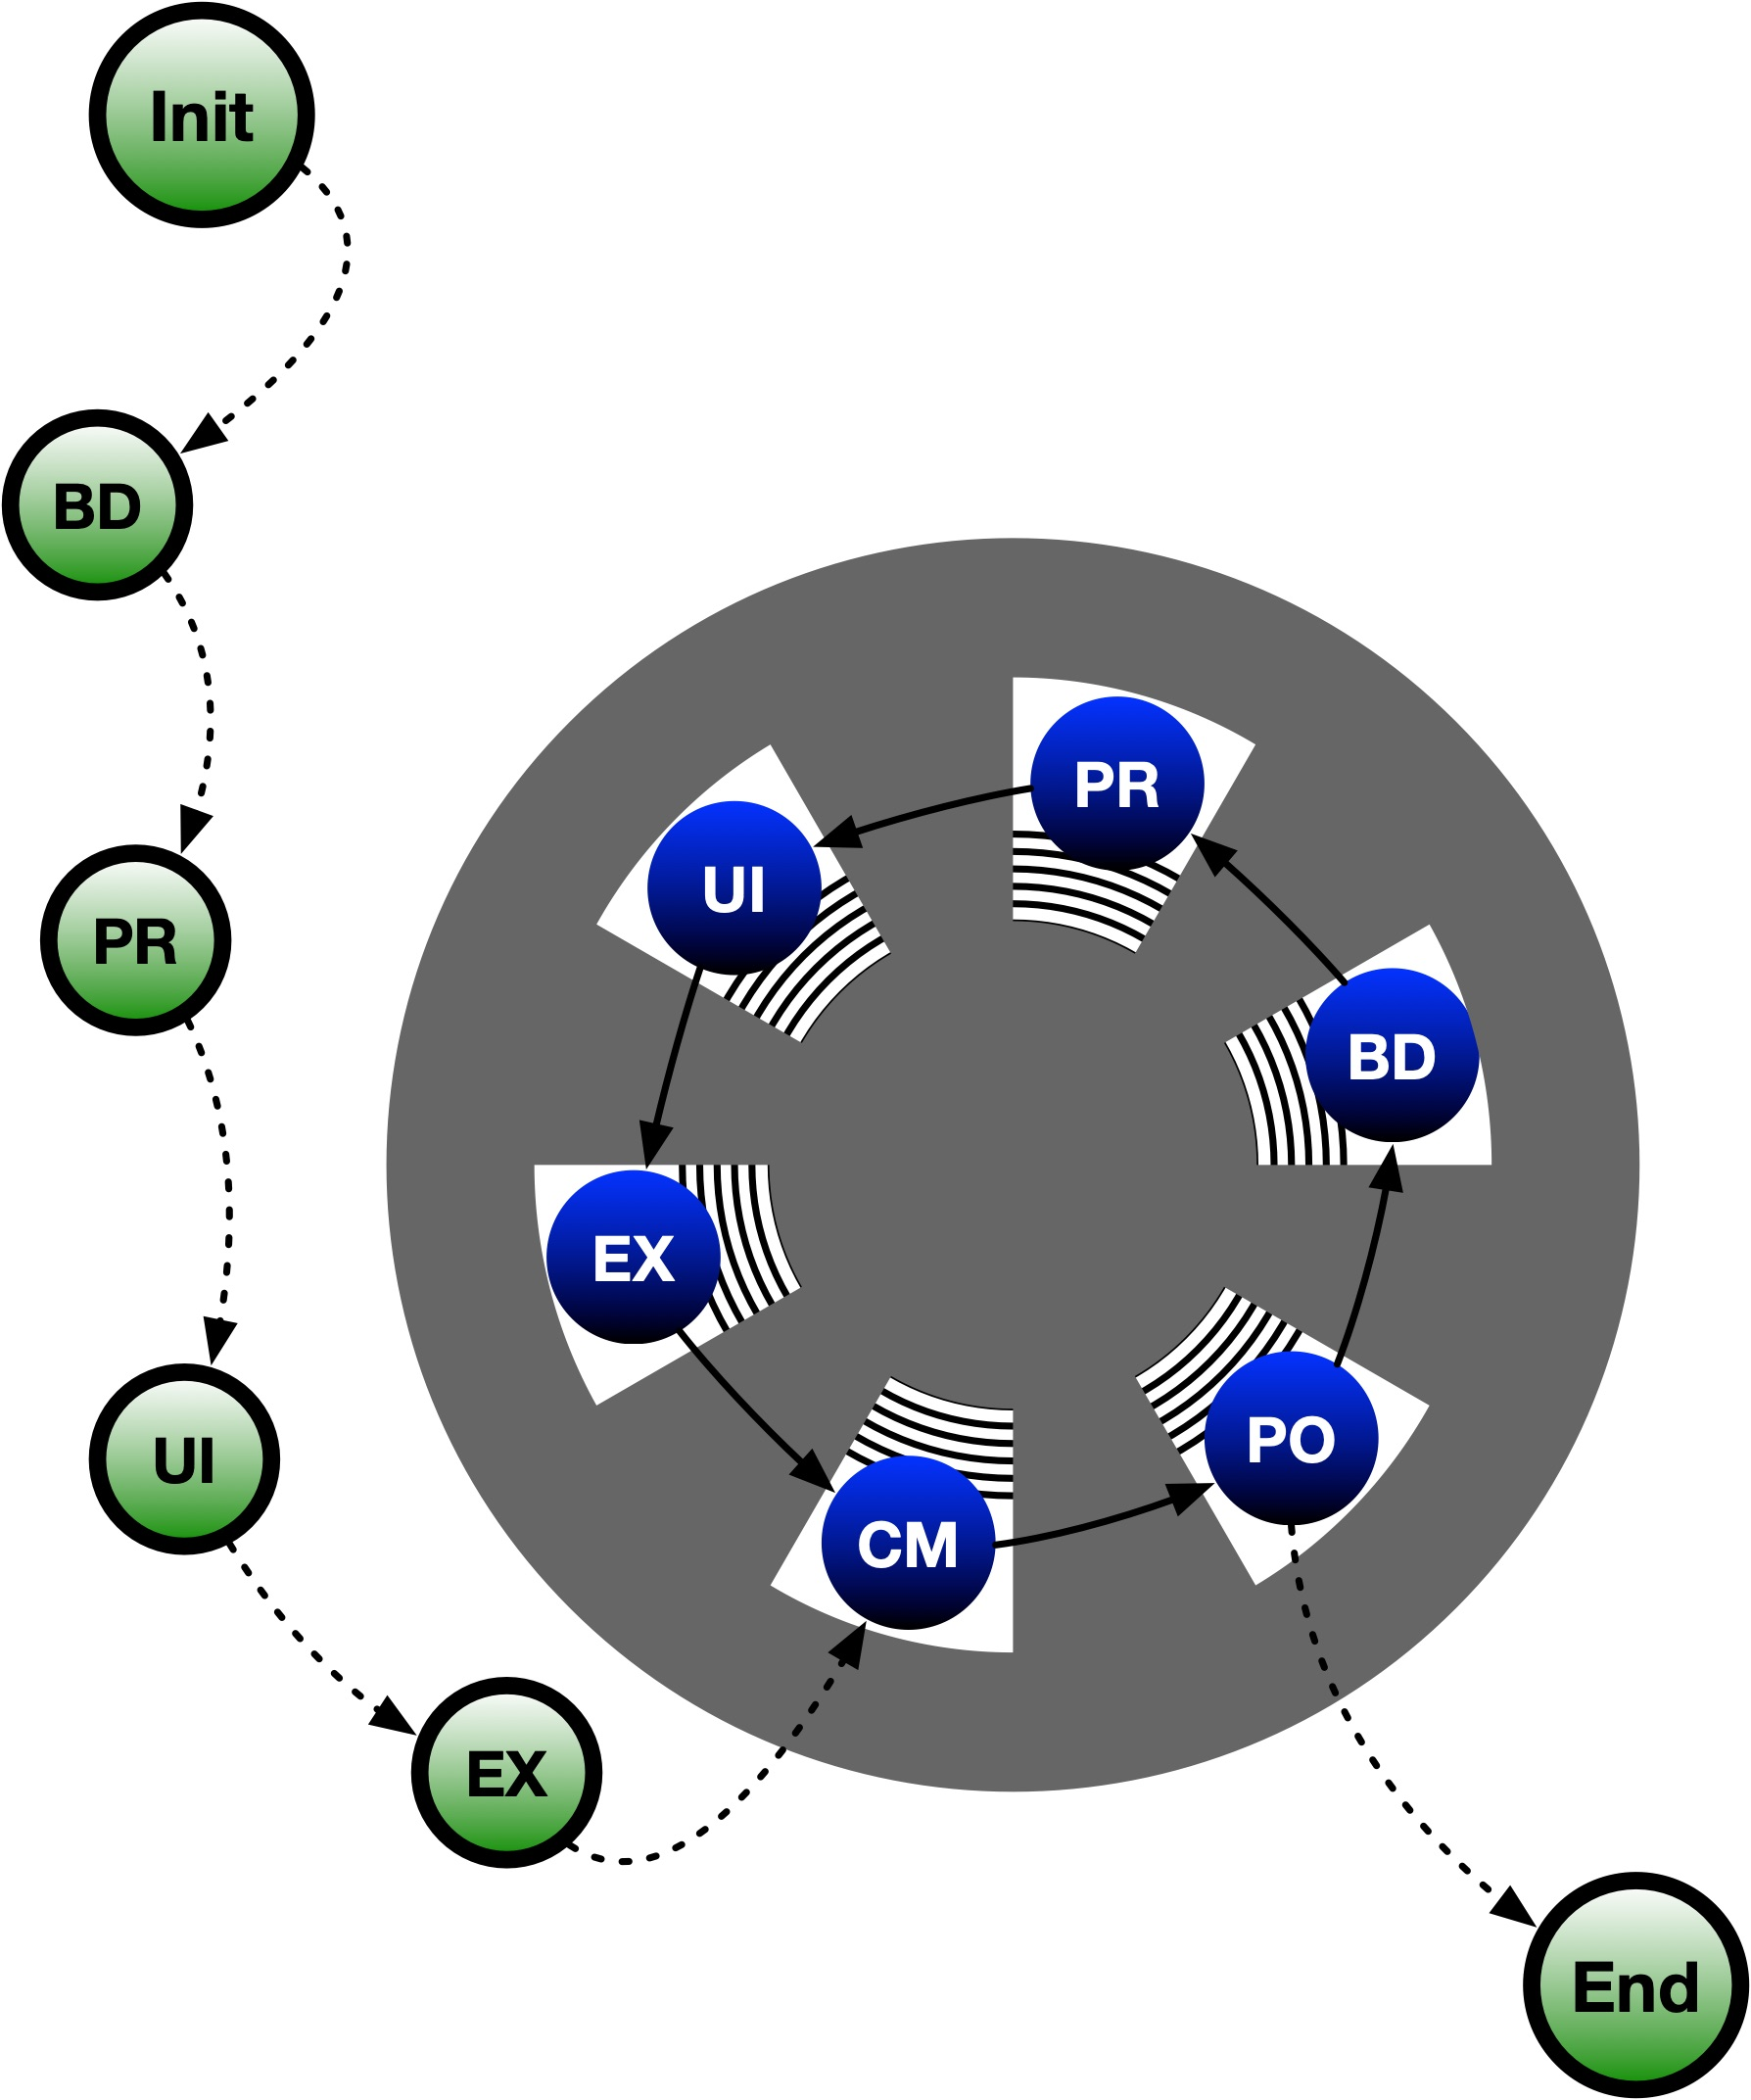
\includegraphics[width=\textwidth]{ferris-wheel.jpg}
        \caption{\label{fig:ferris-wheel-dup-node}}
    \end{subfigure}
    \begin{subfigure}{.3\textwidth}
        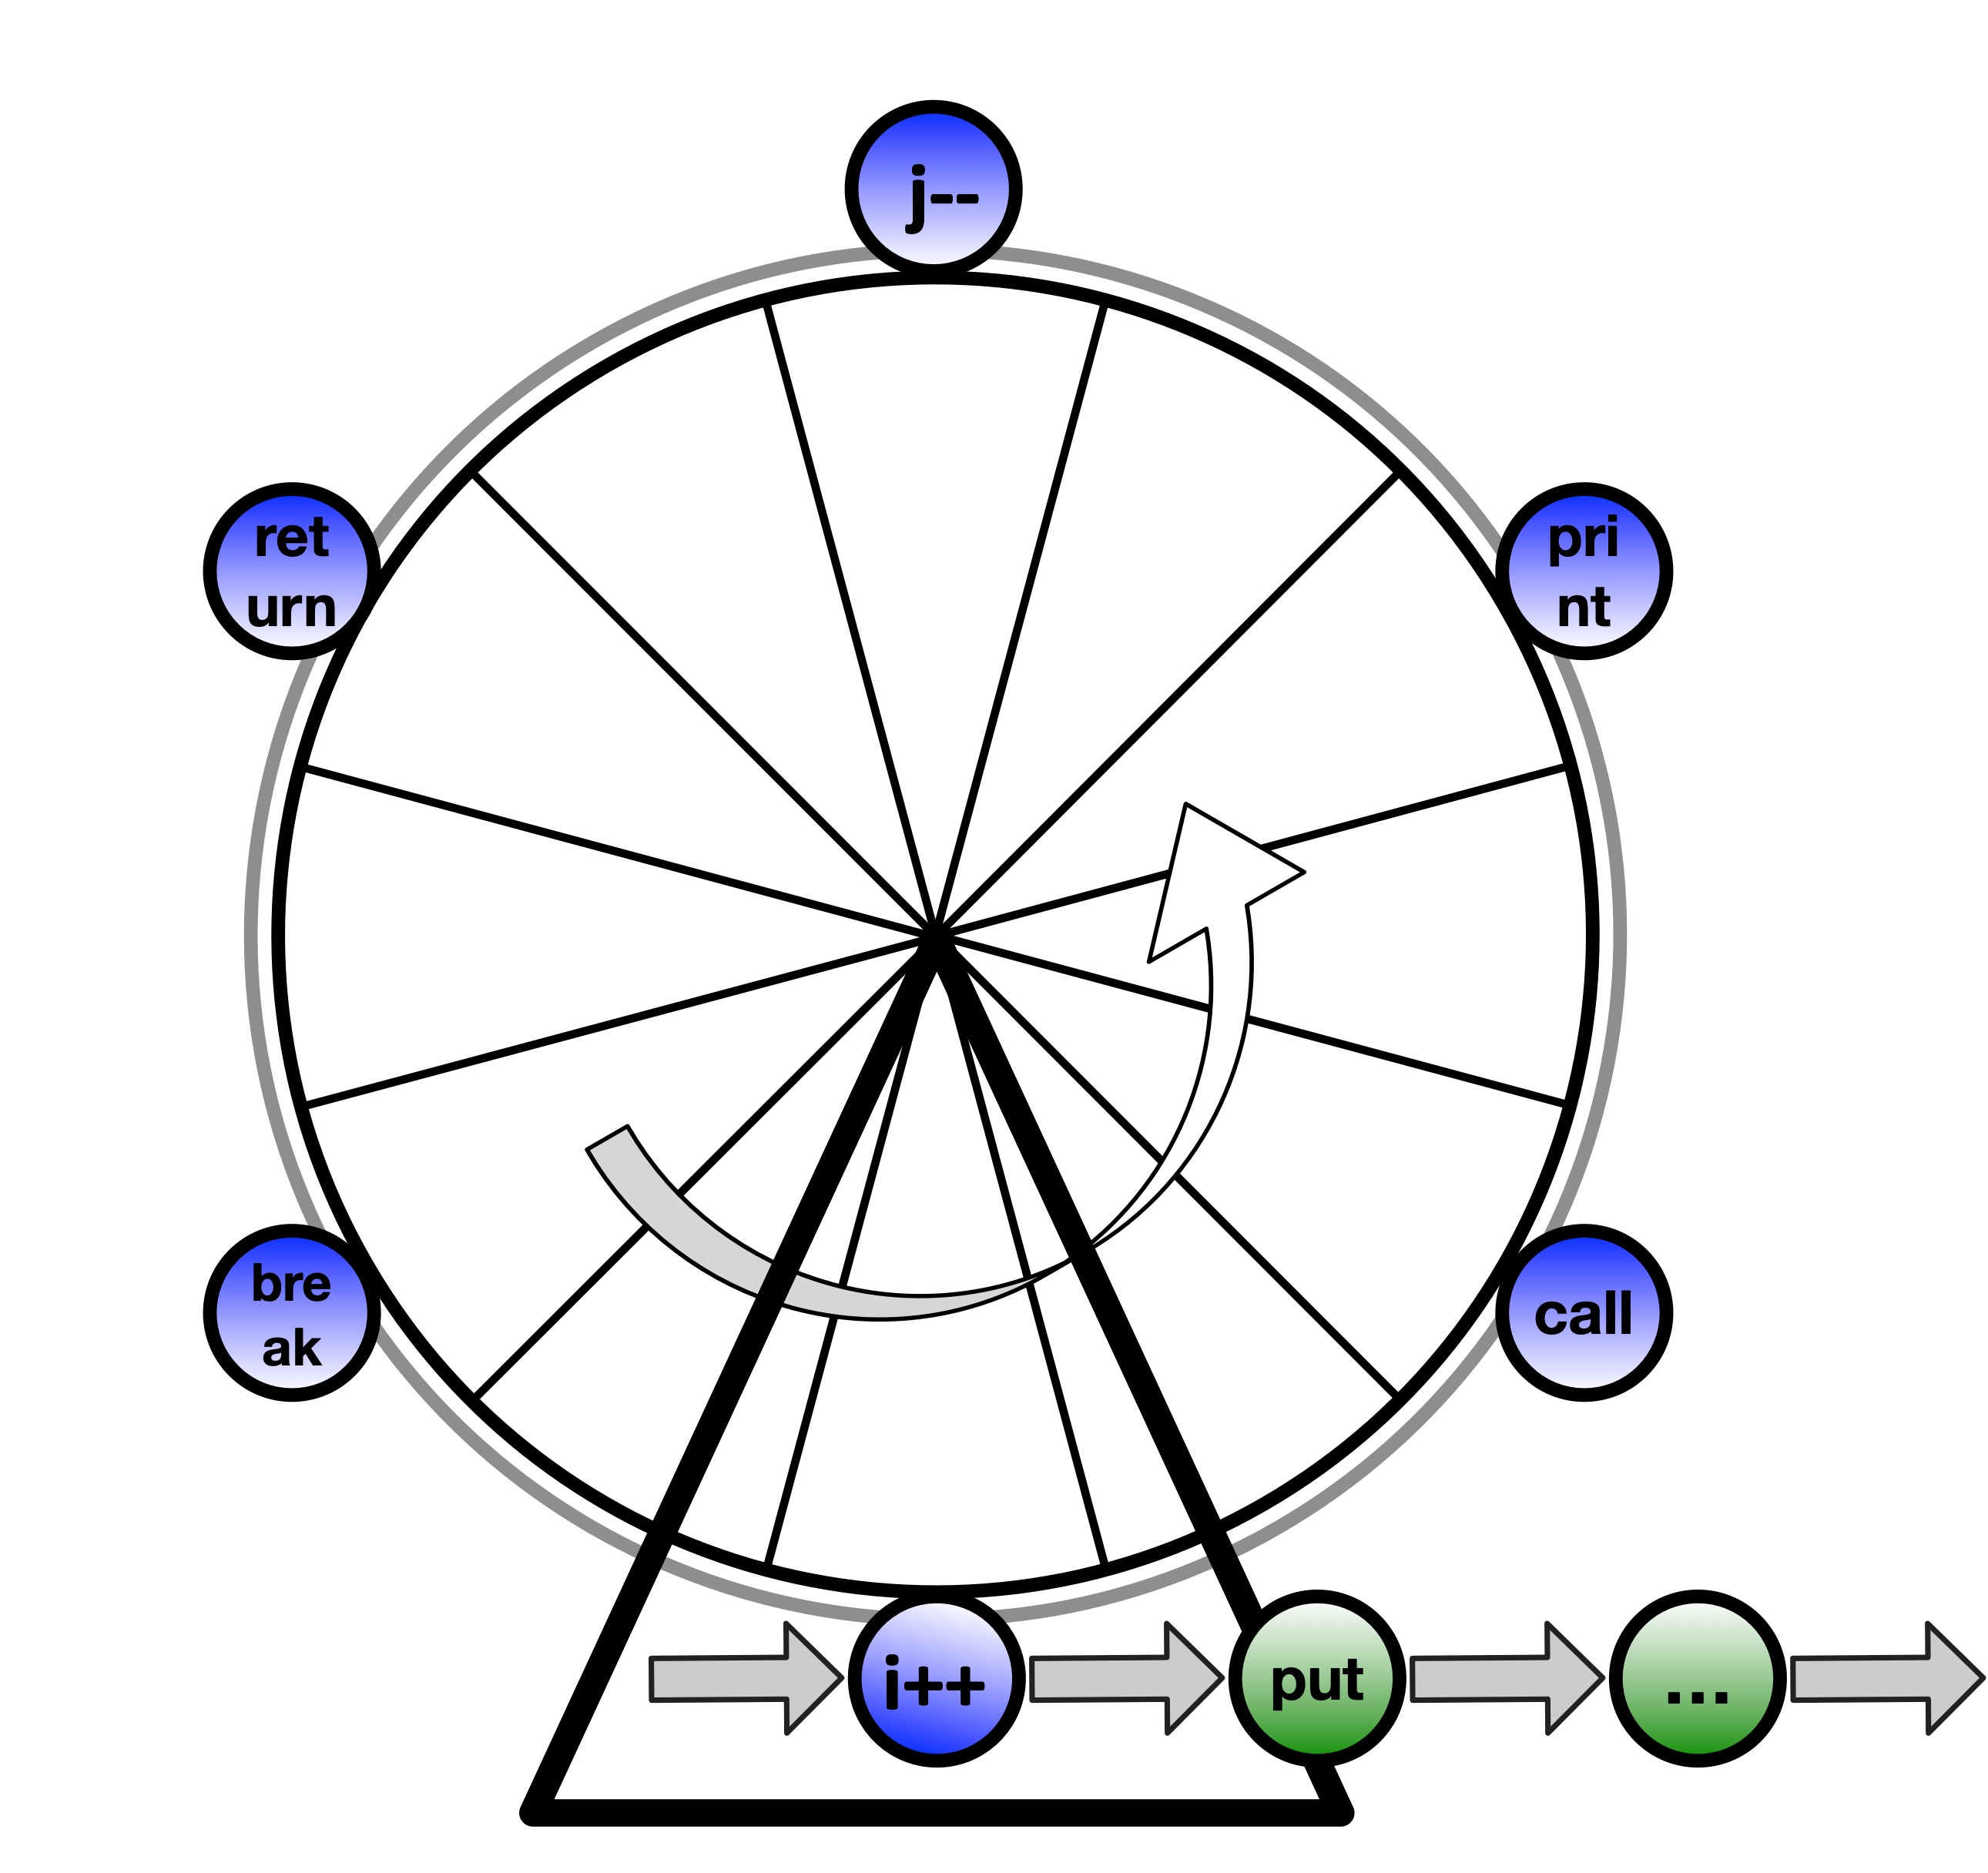
\includegraphics[width=\textwidth]{ferris-wheel-rotated.jpg}
        \caption{\label{fig:ferris-wheel-rotated}}
    \end{subfigure}
    \caption{\label{fig:loop-rotation} Loop as a circular sequence.
    Legend: statements are represented by circular nodes;
    blue ones are loop statements, green ones are non-loop statements.
    The statements ``\code{i++}'' and ``\code{call}'' are duplicated statements between pre-loop
    and loop.
    They can be coalesced into the loop by a loop rotation.
    \protect\subref{fig:ferris-wheel-dup-node}: Original code contains duplicate code;
    \protect\subref{fig:ferris-wheel-rotated}: After rotation, duplicate code is crushed.}
\end{figure}


For example, if the code in the loop and in the vicinity of the loop are duplicate, one may
`rotate' the loop to match up and coalesce the duplicate code.
On the contrary, if one wants to move a portion of the code from the very beginning to the very end
of the loop, one may `reversely rotate' the loop loose.
Doing so will result in duplicate code.
But this may enable a subsequent refactor whose positive effect will eventually pay off this
adverse effect.
In combination, we refer to both operations as `loop rotation'.
In practice, one may start with the more malleable ``\code{while (true)}'' or
``\code{for (; ;)}'' loops.
This will help one focus on coming up with \emph{a} working and flexible code first.
Then one can use the `loop rotation' technique to fine-tune the program.


    \section{Nested Loop thinning Technique}\label{sec:loop-thinning-technique}
    Every developer writes nested loops now and then.
Many times, nested loops appear compelling and inevitable.
While they may solve our problem, nested loops inflict on a program
unnecessary complexity, obstruct code readability, and bring in `soft duplication'.
The presence of nested loops also thwart optimization at the compiler level.
For these reasons, explicit use of loops at high level programming should be avoided
altogether\cite{data-engineering-avoid-loop}.
Moreover, getting rid of nested loops itself may not seem significant improvement.
The optimizations that are made accessible after getting rid of nested loops dwarfs the improvement
brought about by getting rid of nested loops itself.
Like `Candy Crush Saga' game at certain critical point, a single move may unlock an
avalanche of advantageous moves.


In this section, we are to present a process that coalesces nested loops into single-layered loops,
which we will name as `Nested loop thinning technique'.
For sake of argument, the body of the outer loop is divided into three
sections---\emph{pre-inner-loop} section, \emph{inner-loop} section, and
\emph{post-inner-loop} section---depending on their relative position
in respect to the inner loop (as shown in ~\autoref{fig:segment-for-loop-thinning}).
Cramming the functionalities of nested loops into a single loop is no easy task.
As a price, the process almost always results in one or more of the following:
\begin{itemize}
    \item extra conditional constructs
    \item extra tests added to existing conditional constructs
    \item more dynamic loop pacing
    \item more boundary-condition-handling logic
    \item auxiliary data structure, such as queue or stack
\end{itemize}


\begin{figure}
    \centering
    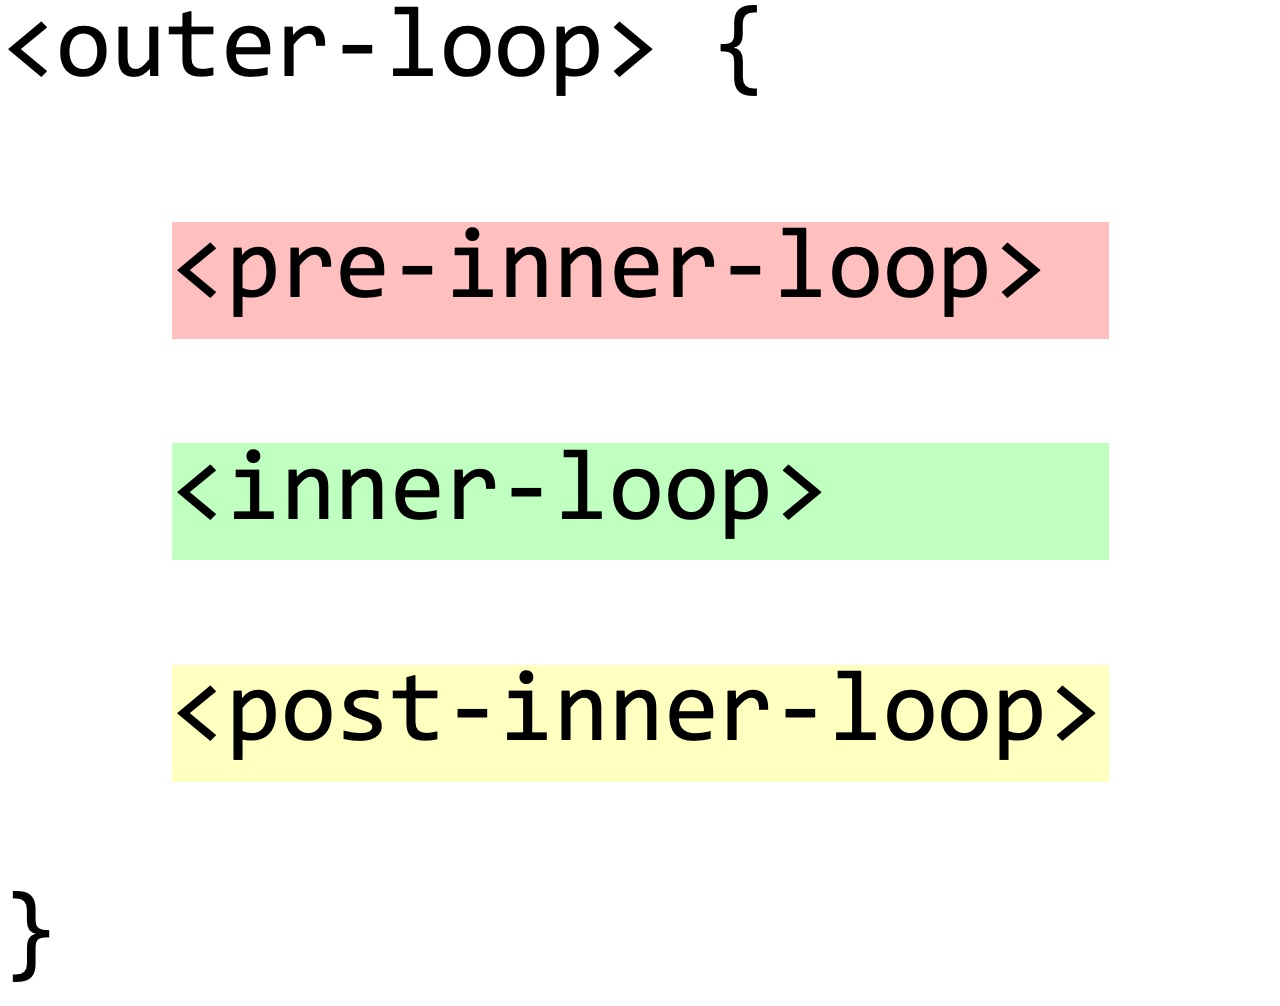
\includegraphics[width=0.4\textwidth]{segment-for-loop-thinning.jpg}
    \caption{\label{fig:segment-for-loop-thinning}
    Sectioning of the body of nested loops:
    \emph{pre-inner-loop} statements, the inner loop itself, and the \emph{post-inner-loop}
    statements.
    Each section receives different treatment during the `nested loop thinning' process.}
\end{figure}


The gist for nested loop thinning process is as follows:
\begin{enumerate}
    \item Preparation stage
    \item Loop rotation to shift around components in the loop body
    \item Reconstruction of loop body using conditionals
\end{enumerate}
But we will go through them one by one.
One will see this pattern again and again for nested loop thinning in practice.


First, some preparatory measures may be taken beforehand
to reduce the friction during the refactor process.
Compound statement is a good example to be dealt with in this step.
Compound statements may get in your way of refactoring for multiple reasons.
The most obvious one is that a compound statement
need to be broken up and sent to different places after refactoring.
State-changing, non-idempotent conditional expressions, such as \code{if (--i < 0)},
are even more lethal because each evaluation of the condition ratchets the state of the loop.
For example,

\begin{minipage}[c]{.3\textwidth}
    \begin{lstlisting}[language=C]
        while (++i < LIMIT);
    \end{lstlisting}
\end{minipage}
\hfill
\begin{minipage}[c]{.3\textwidth}
    shall be expanded to
\end{minipage}
\begin{minipage}[c]{.3\textwidth}
    \lstinputlisting[language=C]{expanded-do-while.java}
\end{minipage}

before the start of loop thinning refactor.
Other types of compound statements, such as \code{if v := a[i]; v < LIMIT}' in Golang, shall be
preprocessed similarly.
Because of the structural similarity between \code{while}-loops and conditionals.
\code{while}-loop readily lends itself to ``nested loop thinning'' process.
For this reason, \code{for}-loop are often converted to \code{while}-loop during preprocessing.


In the second stage, one is to move pre-loop statements, if any, out of the way.
To that end, reverse loop rotation may be used
to unwind the pre-loop statements (see ~\autoref{sec:loop-rotation}).
The second step depends on the inner loop construct.


Finally, it the reconstruction of the loop body using conditional rather than nested loops.
If the inner loop is an unconditional loop as `\code{while True}',
\code{break} statements (or similar) are almost always present and most likely
in a conditional statement somewhere in the loop body unless
it is intended to be a non-typical loop construct.
One should replace the \code{break} statement with the post-inner-loop statements.
The inner loop can then be stripped away.
Otherwise, if the inner loop comes with a non-trivial termination condition,
then the inner loop can be converted to a conditional directly,
\code{while} $\rightarrow$ \code{if},
while the post-inner-loop statements are wrapped away in an \code{else}-clause of it.


Regardless of the venue taken, new conditional statements are inevitably formed or extended
and `cascading conditional construct' are the best way to organize them.
`Cascading conditional construct' consists of ordered sequence of exclusive conditional
statements such as ``\code{if .. elif .. else}''.
For more information, please refer to relevant chapters in Reference ~\cite{Wan:book}.
Throughout the process, one shall pay special attention to execution-path-shunting statements,
such as \code{break} and \code{continue}, if any.


After `nested loop thinning', some cleanup may be performed to comply with convention, code
style, or just for cosmetic reasons.


One disclaimer is that the `nested loop thinning' process does not always prevail.
There are cases where the process is not applicable.
Certain criteria must be met for `nested loop thinning' to be applicable.
First, there must not be intermediate layers, such as
conditional, between the inner and outer loops.
Secondly, execution-path-shunting statements, such as \code{break}, cannot be present in the
pre-inner-loop section.
In what follows, we are going to demonstrate application of `nested loop thinning' technique
on the quicksort algorithms.


    \section{Case Study: quicksort}\label{sec:nested-loop-quick-sort}
    Quicksort is one of the pivotal sorting algorithms widely used by modern software.
First a little background on quicksort.


\subsection{Recursive implementation of quicksort}\label{subsec:recursive-impl-quicksort}
%This is a classical example that was detailed by books such as `Programming
%Pearls' and `Numerical Recipes'\cite{Bentley:1986:PP, NumericalRecipes:1992}.
%My encounter with the code in these books completely redefined the word `simplicity'
%in my dictionary.
%My first implementation of the quicksort algorithm was in C based off
%the traditional ``Hoare's partition scheme'', as presented
%in `Numerical Recipes' (minus the sentinel part).
%But in what follows, I am going to present the idea in Python 2.7.
At the high level, a recursive quicksort implementation may be as follows
\lstinputlisting[label={lst:QuickSortOutline},language=C,
caption={An implementation of quicksort algorithm.}]
{quicksort_outline.c}
where arguments \code{s} and \code{e} are the starting and ending pointers to the input array.
This function invokes `\code{int* part(int* s, int* e)}' which is a function stub for array
partition which will be discussed in detail below.
For single-element arrays, quicksort function is no-op which is a base case.
For na\"{i}ve implementations, this the only base case and it is sufficient.
But for more sophisticated implementations or to reduce partition overhead, more base
cases are used to address under-sized arrays (\textit{e.g.}, arrays of size $\leq 5$ but $\geq 1$).


In plain english, this is how quicksort algorithm works:
\begin{quote}
    If the array contains fewer than $2$ elements (the base case), return as is.
    Otherwise, invoke partition function to partition the array into two subarrays and an
    element (the \emph{pivot}).
    Each subarray is subject to the quicksort function again so on and so forth
    until they are all reduced to the base case.
    At the return of the function, the entire array is sorted.
\end{quote}
The implementation of the partition function is key to the quicksort algorithm.
The partition function does three things:
\begin{enumerate}
    \item Pick a pivot from among the array and set it aside;
    \item Use pivot as a benchmark, partition the rest of the array into two subarrays
    with smaller (or equal) ones on the left and greater (or equal) ones on the right;
    \item Put the pivot element back in between the subarrays.
\end{enumerate}

The subarrays resulted from partition may not be equal sized which is called partition skewness.
Partition skewness has an adverse impact on the performance of quicksort algorithm.
In all practical implementations of the partition function for quicksort, some type of pivot
selection strategy is needed to prevent partition skewness.
Common and proven practices are random selection or ``median-of-three''
technique\cite{sedgewick:1978,sedgewick1977}.
Of course, to apply the ``median-of-three'' technique, the array must exceed a minimum size.


With this said, we are ready to discuss implementation of quicksort and its partition function.
Admittedly, implementing quicksort is quite tricky.
Among the quicksort partition schemes, best known are
Hoare's scheme and Lomuto's scheme\cite{Hoare1961,Bentley:1986:PP}.
The main difference between them lies in how the array is traversed.
In Hoare's scheme, two pointers, one from each end of the array, step toward each other;
whereas in Lomuto's, two pointers, each on its own pace, start off the left end of the array
and step rightward.


Among the quicksort algorithms, there are two main variants---those
by Tony Hoare and by Nico Lomuto, respectively.
Hoare's quicksort scheme has robust and optimal performance but its
implementation has been quite involved.
Lomuto's scheme, on the other hand, is straightforward to implement and easier to follow.
However its performance may degrade catastrophically for certain edge cases.
Comparing the two,
one cannot help but wonder if there is an implementation
that is as robust and performant as the traditional implementation of Hoare's quicksort algorithm
and at the same time as succinct as that of Lomuto's.
That is going to be the focus of rest of this article.


\subsection{Implementation of Lomuto's Partition Scheme}\label{subsec:impl-of-Lomuto-part-fun}

\lstinputlisting[label={lst:singleLoopLomuto},language=C,
caption={Implementation of Lomuto's partition scheme for quicksort.}]
{quicksort_partition_asym.c}
Let's start with the relatively simpler Lomuto's partition scheme.
In Lomuto's partition scheme, the two pointers have distinct tasks.
The one running in front, variable \code{i}, is responsible to discover out-of-place elements.
The one behind, \code{p}, guards the partition boundary.
When \code{i} discovers an out-of-place element, \code{p} makes
room and places it by a swap and the partition process continues.
The code is shown in ~\autoref{lst:singleLoopLomuto}.
Once one understands the code, implementation becomes highly consistent and intuitive.
One seldom fails implementing even for a customized applications.


Notably, implementing this partition scheme only needs one loop.
However the simplicity is no free lunch.
In fact, for certain edge cases, Lomuto's partition scheme suffers severe performance penalty,
\texttt{e.g.}, arrays with a large number of identical elements,
in which the Lomuto's quicksort algorithm degrades close to quadratic runtime.
The root cause leading to this degradation lies in the asymmetric traversal of the array which
inevitably leads to partition skewness.
With the Lomuto's quicksort partition function, let's come back and study the more sophisticated
implementation---the symmetric Hoare's partition scheme.


\subsection{Implementation of Hoare's Partition Scheme}\label{subsec:impl-of-qsort-part-fun}

Invented along with the quicksort algorithm, the Hoare's partition scheme predates Lomuto's
historically\cite{Hoare1961,Hoare1962,sedgewick:1978}.
Because of its symmetric traversal, Hoare's partition scheme successfully avoids the drawback of
Lomuto's.


Visually speaking, Hoare's partition scheme employs two pointers, \code{s} and \code{e}, starting
off the opposite ends of the array, push through the array toward each other,
given that a pivot element has been placed at the beginning of the array.
As in Lomuto's partition function, these pointers also stop at `out-of-place' elements.
When both stop, the `out-of-place' elements are swapped to where they belong.
Then the pointers are on their way again so on and so forth until they meet or cross.
At last the pivot element is swapped into its final position and a pointer to this final position
is returned.


While it appears a minor change from Lomuto's scheme, the Hoare's partition comes with immense
implementation complexity.
%The above description of Hoare's partition scheme disguises the true complexity of
%implementing it.
So much so that for a long time how Hoare's partition scheme work
remained an enigma\cite{Bentley-Beautiful-code}.
There are so many changing variables and so much coupling among them that once in a
while, each attempt of implementing it may end up with a different solution.
Even worse than that, when something goes wrong, one is often clueless as to what is wrong.
Also, it is extremely hard, if not impossible, to devise a test case to hit an elusive bug.


But in stark contrast to the numerous slightly differing implementations, all known implementations
have so far unanimously used $3$ nested loops: one outer loop and two sequential inner loops.
This feature is so commonplace that it has become the sterotype of quicksort.



%In C-like language when it comes to intervals bound by pointers,
%there are two semantically distinct conventions.
%One is inclusive beginning and exclusive end, the 'close-end' convention.
%The other is inclusive for both boundaries, the 'close-close' convention.
%Correspondingly, quicksort implementations fall in two categories, one for each convention.
%There are renowned computer scientists who advocate one over the other\cite{dijkstra-ewd831}.
%But for quicksort, .


With the Hoare's partition scheme, a commonly found implementation for the partition function is as
follows.
\lstinputlisting[label={lst:nestedLoopHoareMethod},language=C,
caption={Implementation of Hoare's partition scheme for quicksort.}]
{quicksort_partition_sym.c}
While we have given an outline of the working of Hoare's partition, many choices remain to be
made in regard of ``how, when, and what''.
As such, pitfalls lay in wait every now and then throughout the implementation process.
We will leave the discussions of the implementation process of ~\autoref{lst:nestedLoopHoareMethod}
encountered during this implementation in ~\autoref{sec:impl-varieties}.


\subsection{Removal of the Nested Loops}\label{subsec:unwind-hoare-part}

Now we are going to use the techniques presented earlier to transform the traditional
implementation of Hoare's partition scheme and get rid of the nested loops.


The immediate difficulty is how to take apart the densely packed conditional construct:
\begin{lstlisting}
    while(s < e && *++s < *pivot);
    while(pivot < e && *--e > *pivot);
\end{lstlisting}
The loop conditions here are unusual and awkward to handle
because both `\code{++s}' and `\code{--e}' ruthlessly ratchet the loop state forward
whenever control is passed to this line.
Namely, each evaluation of the loop condition, even if the condition evaluates to false, the
pointers `\code{s}' and `\code{e}' are still incremented.
If we use these conditions as is in the to-be conditional constructs, we would end up in a
dilemma---when we discover out-of-place elements, we would pass them without swap in the next
iteration because the program does not leave us any chance for that.
With the existing programming languages' syntaxes, we have no choice but to break
up the pre-incremental statements.
So something must be done to unfold the extraordinary loop conditions to
ordinary ones before we proceed with the rest of the `nested loop thinning' procedure.
As we learned in ~\autoref{ch:loops}, these loops may be converted first to
`\code{do-while} loops' such as
\lstinputlisting[language=C]{quicksort_inner_loop_do_while.c}
and the latter are, in turn, converted to `\code{while} loops':
\lstinputlisting[language=C]{quicksort_inner_loop_while.c}
After these changes are applied, our the partition function becomes
\lstinputlisting[language=C]{quicksort_partition_sym_expanded_inner_loop.c}
You may have noticed that we have floated ~\code{--e} up in front of the first inner loop,
and this does not affect the correctness as can be verified.
The solution now seems equally messy, if not more so, as we started.
However, as you will see, this form will prove useful for the subsequent refactor step---`loop
rotation'.
Now we can proceed with the next step
of loop thinning---move the \emph{pre-inner-loop statements} out of the way.
(``Loop rotation'' is specified in ~\autoref{sec:LoopDesignConsideration}.)
After this step, the code becomes:
\lstinputlisting[language=C]{quicksort_partition_sym_rotated_inner_loop.c}
We have accelerated the process by tucking the \emph{post-inner-loop statements}
resulted from the loop rotation to a conditional block.
Now we are ready with the third and most exciting step---converting inner loops to conditionals.
Now we encounter a complication that is new to us: we need to covert the second loop to an
`\code{else if}' clause of the first because the second inner loop is executed only after the first
exits.
Our final result is posted below after the conversion to conditional construct:
\lstinputlisting[label={lst:singleLoopHoarePart},language=C,escapechar=\$,
caption={Implementation of partition function for Quicksort using one loop.}]
{quicksort_partition_single_loop.c}
Note that we have combined multiple statements into a compound one `~\code{swap(s++, e--)}'.
%By now we conclude our ``nested loop thinning' refactor process.
By now,
we achieved our goal of a partition implementation that has the simplicity of
Lomuto's and the robust performance of Hoare's.
In retrospection, we set off to test the hypothetical quest for a simple but performant
partition scheme that comprises the advantages of Lomuto's and Hoare's partition scheme.
Comparing with where we started off ~\autoref{lst:nestedLoopHoareMethod},
we implemented the Hoare's algorithm with a single loop plus
cascading conditionals as ~\autoref{lst:singleLoopHoarePart}.
In the process, we used the `loop rotation' techniques, the `nested loop thinning' techniques,
and skills concerning the construction of cascading conditionals from earlier sections.
The new quicksort implementation retains the optimal runtime as Hoare's algorithm but has
comparable simplicity as that of Lomuto's.
That's almost too good to be true!
%If this does not impress you, then you have no feeling.
While we can make the solution simpler with the use of sentinel, we will leave that discussion to
next section.
However there is one change that can provide a little more saving.
If we change the semantic of ending pointer \code{e} from exclusive to inclusive, the
pre-increment before the loop (line~\ref{quicksort:pre-increment} of
~\autoref{lst:singleLoopHoarePart}) would be unnecessary.
As a byproduct of going through the detailed refactor
processes for the cases of this section, I want the reader to have a feeling about software
development model.
As we can see the most fruitful software development model, undoubtedly, is to come up with a
working solution first.
However shabby, messy, primitive a solution it may be, as long as it can pass a handful of unit
tests, it will be a great starting point.
Then through meticulous optimization process, for which many of the techniques we have talked
about and will be talking may be an aid, strive for straightforwardness, simplicity, and elegance.
In the course, one may discover new issues, adding new unit tests accordingly, and obtain new
solutions.
With the variety of solutions passing the same unit tests, one can often form a better
perspective regarding the solution space.
This will help one pick the most effective solution to the original problem.
%This is as a general programming guideline as well as specific  ally applicable to loops.

\section{Sentinels in quicksort}\label{sec:quick-sort-sentinel}
%TODO Simplify the presentation of sentinels to one to two sentences

The cascading conditional in the loop body of ~\autoref{lst:singleLoopHoarePart}
is still far from straightforward.
A further simplification on that may achievable through the use of
sentinels~\cite{NumericalRecipes:1992}.

%It was eye-opening to see how the authors gracefully avoided the array boundary checks
%with the use of sentinels.
%I psychologically accepted the pitch made for sentinels while I was with the book.
%Closing the book, however, I am still dubious about its plausibility until I myself have a
%success implementing it.
%In this section, I pick this work to make a pitch to the reader about sentinels.


For stark effect of the sentinels, we will first fix the traditional implementation of `Hoare's
partition scheme':
~\autoref{lst:QuickSortOutline} gives the outline of the program and
~\autoref{lst:nestedLoopHoareMethod} gives a fully implemented partition function.
As mentioned earlier, one can get involved in the thick of implementing
`Hoare's quicksort algorithm'.
Not only the problem itself is tricky but also the way we implement it.
By picking Hoare's quicksort scheme over its alternative (such as Lomuto's),
we insist on the robust $O(N log N)$ expected runtime.


We attempt to get rid of the boundary checking using sentinels.
These boundary checking are there to ensure that the pointers `\code{s}' and `\code{e}' do not slip
off the ends of the array.
In large arrays, these boundary check operations may get in the way of performance of the algorithm.
But the main reason of doing so is to remove clutter in the code.
%For another, we are consciously attacking the problem with an precautions approach against
%performance degradation so there is a price we have to pay.

The main idea is to make boundary checking redundant by effecting some artifacts that catch the
pointers before the `out of boundary' error happens.
This is exactly what sentinel is good at!
By deploying sought-after values, the `sentinels', at the ends of the array before the control
hits the loop, the following will happen:
\begin{enumerate}
    \item the pointers, `\code{s}' and `\code{p}', would have to stop when they hit the ends of
    array;
    \item the subsequent logic will guarantee the termination of the outer loop and
    thus guarantee the inner loop would not be executed again.
\end{enumerate}


What are the sought-after values by `\code{s}' and `\code{e}'?
The out-of-place values!
Particularly, \code{s} is looking for values that are `$\geq$ the pivot';
\code{e} is looking for values `$\leq$ the pivot'.
So then instead of randomly picking one value for pivot, we now randomly pick $3$ values, the median
of which be elected as the pivot as usual, the minimum be deployed to the left end, and the maximum
to the right end.
We group these operations into a function called `\code{init_swap}':
\lstinputlisting[]{qsort_init_swap.c}


Now back the function `\code{part}'.
As we mentioned before, the deployment of sentinels in function `\code{init_swap}' makes
the conditional expressions `\code{s < e}' and `\code{pivot < e}' semantically redundant.
They can now be safely removed.
Below is the function `\code{part}' after all the refactoring is done.
\lstinputlisting[]{qsort_part_sentinel.c}
Comparing with the implementation ~\autoref{lst:nestedLoopHoareMethod}, this code
cleans out clutter in the loop conditions in the inner loops.
We `float' the control all the way through the termination of the program on a `touchless' rail made
by sentinels, without ever needing to check boundary condition.
Of course, the onus is shifted to the initialization before the loop.
Comparing with the inner loops, that section is non-critical.
Not only that the code is made less cluttered, but also the number of such checks
is reduced from $O(N)$ to $O(1)$.
More importantly, by not checking boundary conditions at the most critical section,
we avoid bugs that would otherwise cost us many hours of debugging time.


So by use of sentinels on the traditional Hoare's quicksort algorithm,
we shifted the complexity among the nested loops to a non-critical part of the program,
effectively reduced its coding complexity.
Remember that we came up with a new, single-loop implementation for the Hoare's quicksort algorithm
in ~\autoref{ch:loop-thinning}, as presented in ~\autoref{lst:singleLoopHoarePart}.
Can we apply the idea of sentinel to make it even better?
Yes, it may be applied equally well.
Below is the implementation of the function `\code{part}' with a single loop and simplified
boundary condition with sentinel values.
\lstinputlisting[]{quicksort_partition_single_loop_sentinel.c}
This brings implementations of Hoare's quicksort to the next level of simplicity.


    \section{Experiment}\label{sec:experiment}
    In all the quicksort implementations in this article, we use the
``median-of-three'' pivot selection technique to prevent pivot skewness
\code{part}\cite{sedgewick1977,sedgewick:1978}.
Correspondingly, we ensure that the array length is at least $3$ to call function \code{part}.

\begin{table}[b]
    \centering
    \caption{\label{tab:quicksort-experiment}
    Runtime measurement of Hoare's quicksort algorithms,
    comparing the traditional implementation and the single-loop implementation.
    Experiments are run against three data sets---the first is sorted ascending,
    the second descending, and the third is randomly ordered.
    Courtesy: The experiment is conducted based on project ``Benchmarking Sorting
    Algorithms''\cite{benchmarking-sorting-algo} with some modification.}
    \vskip 10pt
    \begin{tabular}{r|r|r|r}
        \hline
        \multicolumn{4}{l} {\mbox{Integer arrays in ascending order}}\\
        array size & Traditional & Simplified & Percent difference\\
        \hline
        $10$ & $7$ & $8$ & $14\%$\\
        $100$ & $18$ & $20$ & $11\%$\\
        $1,000$ & $111$ & $126$ & $14\%$\\
        $10,000$ & $1,071$ & $1,239$ & $16\%$\\
        $50,000$ & $4,893$ & $5,867$ & $20\%$\\
        $100,000$ & $9,479$ & $11,131$ & $17\%$\\
        $1,000,000$ & $115,248$ & $137,658$ & $19\%$\\
        \hline
        \multicolumn{4}{l} {\mbox{Integer arrays in descending order}}\\
        array size & Traditional & Simplified & Percent difference\\
        \hline
        $10$ & $7$ & $7$ & $0\%$\\
        $100$ & $18$ & $19$ & $6\%$\\
        $1,000$ & $106$ & $142$ & $34\%$\\
        $10,000$ & $1,020$ & $1,167$ & $14\%$\\
        $50,000$ & $4,757$ & $5,411$ & $14\%$\\
        $100,000$ & $9,378$ & $11,132$ & $19\%$\\
        $1,000,000$ & $118,696$ & $138,311$ & $17\%$\\
        \hline
        \multicolumn{4}{l} {\mbox{Integer arrays randomly ordered}}\\
        array size & Traditional & Simplified & Percent difference\\
        \hline
        $10$ & $6$ & $6$ & $0\%$\\
        $100$ & $25$ & $25$ & $0\%$\\
        $1,000$ & $264$ & $249$ & $-6\%$\\
        $10,000$ & $2,949$ & $3,065$ & $4\%$\\
        $50,000$ & $16,565$ & $17,943$ & $8\%$\\
        $100,000$ & $34,005$ & $36,400$ & $7\%$\\
        $1,000,000$ & $380,477$ & $406,659$ & $7\%$\\
        \hline
    \end{tabular}
\end{table}

~\autoref{tab:quicksort-experiment} shows the runtime analysis and comparisons.
The simplified implementation indeed comes with an overhead and is thus slower than
its traditional counterpart of the Hoare's quicksort program.
For sorted data sets (either ascending or descending), there is a $17\%$ slowdown.
But for randomly ordered data sets, the slow down is consistantly around $7\%$.
The experiment data seems to indicate that the simplified
implementation of Hoare's quicksort algorithm shares same runtime complexity as its
traditional counterpart.
Their performance may differ by a multiplier.


    \section{Conclusion}\label{sec:conclusion}
    In this article, we presented a couple of techniques for optimizing loop constructs in
    high-level programming languages.
    Taking advantage of the circular symmetry of loop constructs, loop rotation may be applied to a
    loop to either reduce code duplication (forward rotation) or to shift certain part of the
    code within the loop body (reverse rotation).
    Another technique is loop thinning for simplifying nested loop complications.
    These are two of the empirical techniques that helps programmers achieve software development
    best practices.
    As an example, we applied these techniques in simplifying a traditional implementation of
    Hoare's quicksort algorithm.
    We provided the simplified implementation in C++.
    More generally, the programming techniques we developed in this article are applicable to all
    programming languages that supports loop and conditional constructs.
    \begin{appendices}
        \appendix
        %%
%% Author: shoupu_wan
%% 2019-04-13
%%
\appendix{Hoare's Partitioning Functions}\label{apx:impl-varieties}

\lstinputlisting[label={lst:part_nested_loop_var1},language=C,
caption={Partition scheme for quicksort variation 1.
For elements equal to the pivot, we don't stop '<=' or '<' is not critical.
But '<=' brings more saving on unnecessary swaps.}]
{part_nested_loop_var1.c}

\lstinputlisting[label={lst:part_nested_loop_var2},language=C,
caption={Partition scheme for quicksort variation 2.
Found another variation of partition scheme based on part-nested-loop
Diff wise, it lies between part-nested-loop and part-nested-loop-var
- the order of the two while loops is identical to part-nested-loop
- the boundary checking is identical to part-nested-loop-var
- the return value is shifted toward the left by one unit
}]
{part_nested_loop_var2.c}

\lstinputlisting[label={lst:part_nested_loop_var3},language=C,
caption={Partition scheme for quicksort variation 3.
Variation of partition scheme.
The two differs in three ways
- order of the two while loops
- increment condition for equal element pointer
- return pointer choice between s and e
}]
{part_nested_loop_var3.c}

\lstinputlisting[label={lst:part_nested_loop_var4},language=C,
caption={Partition scheme for quicksort variation 4.
Find yet another variation of implementation where the second nested while-loop
is made post-incremental.
This will remove the difficulty encountered in loop-thinning.}]
{part_nested_loop_var4.c}

All these listings are to be understood with some pivot-selection mechanism to avoid pivot
skewness.

\appendix{Quicksort Partitioning function in Go}\label{apx:partition-go}

        %%
%% Author: shoupu_wan
%% 2019-05-22
%%

\section{Sentinels in quicksort}\label{sec:quick-sort-sentinel}
%TODO Simplify the presentation of sentinels to one to two sentences

The cascading conditional in the loop body of ~\autoref{lst:singleLoopHoarePart}
is still far from straightforward.
A further simplification on that may achievable through the use of
sentinels~\cite{NumericalRecipes:1992}.

%It was eye-opening to see how the authors gracefully avoided the array boundary checks
%with the use of sentinels.
%I psychologically accepted the pitch made for sentinels while I was with the book.
%Closing the book, however, I am still dubious about its plausibility until I myself have a
%success implementing it.
%In this section, I pick this work to make a pitch to the reader about sentinels.


For stark effect of the sentinels, we will first fix the traditional implementation of `Hoare's
partition scheme':
~\autoref{lst:QuickSortOutline} gives the outline of the program and
~\autoref{lst:nestedLoopHoareMethod} gives a fully implemented partition function.
As mentioned earlier, one can get involved in the thick of implementing
`Hoare's quicksort algorithm'.
Not only the problem itself is tricky but also the way we implement it.
By picking Hoare's quicksort scheme over its alternative (such as Lomuto's),
we insist on the robust $O(N log N)$ expected runtime.


We attempt to get rid of the boundary checking using sentinels.
These boundary checking are there to ensure that the pointers `\code{s}' and `\code{e}' do not slip
off the ends of the array.
In large arrays, these boundary check operations may get in the way of performance of the algorithm.
But the main reason of doing so is to remove clutter in the code.
%For another, we are consciously attacking the problem with an precautions approach against
%performance degradation so there is a price we have to pay.

The main idea is to make boundary checking redundant by effecting some artifacts that catch the
pointers before the `out of boundary' error happens.
This is exactly what sentinel is good at!
By deploying sought-after values, the `sentinels', at the ends of the array before the control
hits the loop, the following will happen:
\begin{enumerate}
    \item the pointers, `\code{s}' and `\code{p}', would have to stop when they hit the ends of
    array;
    \item the subsequent logic will guarantee the termination of the outer loop and
    thus guarantee the inner loop would not be executed again.
\end{enumerate}


What are the sought-after values by `\code{s}' and `\code{e}'?
The out-of-place values!
Particularly, \code{s} is looking for values that are `$\geq$ the pivot';
\code{e} is looking for values `$\leq$ the pivot'.
So then instead of randomly picking one value for pivot, we now randomly pick $3$ values, the median
of which be elected as the pivot as usual, the minimum be deployed to the left end, and the maximum
to the right end.
We group these operations into a function called `\code{init_swap}':
\lstinputlisting[]{qsort_init_swap.c}


Now back the function `\code{part}'.
As we mentioned before, the deployment of sentinels in function `\code{init_swap}' makes
the conditional expressions `\code{s < e}' and `\code{pivot < e}' semantically redundant.
They can now be safely removed.
Below is the function `\code{part}' after all the refactoring is done.
\lstinputlisting[]{qsort_part_sentinel.c}
Comparing with the implementation ~\autoref{lst:nestedLoopHoareMethod}, this code
cleans out clutter in the loop conditions in the inner loops.
We `float' the control all the way through the termination of the program on a `touchless' rail made
by sentinels, without ever needing to check boundary condition.
Of course, the onus is shifted to the initialization before the loop.
Comparing with the inner loops, that section is non-critical.
Not only that the code is made less cluttered, but also the number of such checks
is reduced from $O(N)$ to $O(1)$.
More importantly, by not checking boundary conditions at the most critical section,
we avoid bugs that would otherwise cost us many hours of debugging time.


So by use of sentinels on the traditional Hoare's quicksort algorithm,
we shifted the complexity among the nested loops to a non-critical part of the program,
effectively reduced its coding complexity.
Remember that we came up with a new, single-loop implementation for the Hoare's quicksort algorithm
in ~\autoref{ch:loop-thinning}, as presented in ~\autoref{lst:singleLoopHoarePart}.
Can we apply the idea of sentinel to make it even better?
Yes, it may be applied equally well.
Below is the implementation of the function `\code{part}' with a single loop and simplified
boundary condition with sentinel values.
\lstinputlisting[]{quicksort_partition_single_loop_sentinel.c}
This brings implementations of Hoare's quicksort to the next level of simplicity.

    \end{appendices}
    \bibliographystyle{unsrt}
    \bibliography{main}
\end{document}
